\scanpage{151}
$\underline{\Sigma}=(X,\Sigma)$, d'où surface cellulaire des positions relatives $X^*=\operatorname{Rel}(\underline{\Sigma})$.

Soit un sommet \inserted{$\rho$} de $X^*$, correspondant à une position relative critique \deleted{$\unsure{\Delta}$}$D_{\rho}$, soit $S_{\rho}=D_{\rho}\cap S(\Sigma)$.
\inserted{Une orientation $\unsure{\bar\omega}$ de $X^*$ correspond à une orientation $\bar\omega_{\rho}$ de $D_{\rho}$.}
Alors les \unsure{arcs sort.} de $\rho$ de $X^*$ correspondent aux \deleted{\unsure{somm.}} éléments \inserted{$(s,\omega)$} de $S_{\rho}$, \uline{munis} d'une orientation; \inserted{soit $\vec a_{s,\omega}$ l'arc}.
A un tel couple $(s,\omega)$, correspond la pos. semi-stble $(D_{\rho},s,\omega)$ \deleted{\unsure{orientée}\ \unsure{qui}} ,
\deleted{\unsure{qui provient}\ \unsure{définit l'arc}\ \unsure{dans le voisin}\ \unsure{germes} $(\rho,\unsure{\bar\omega})$ \unsure{correspond. à une} p.r. stble}
à l'arête $a_{s,\omega}$ sous-jacente : $\vec a_{s,\omega}$; soit $\vec b_{s,\omega}$ l'arête duale, orientée de façon que $(\vec a_{s,\omega},\vec b_{s,\omega})$ soit direct pour $\unsure{\bar\omega}$, donc $\vec b_{s,\omega}$ va d'une p.r. \uline{stable} vers une autre -- c'est le passage de la \unsure{générisation} de $D_{s,\omega}$ en $s$ dite ``\unsure{gauche}'' vers la gén. \unsure{vue|dite} \deleted{\unsure{gauche}}\inserted{\uline{droite}}.
\figure{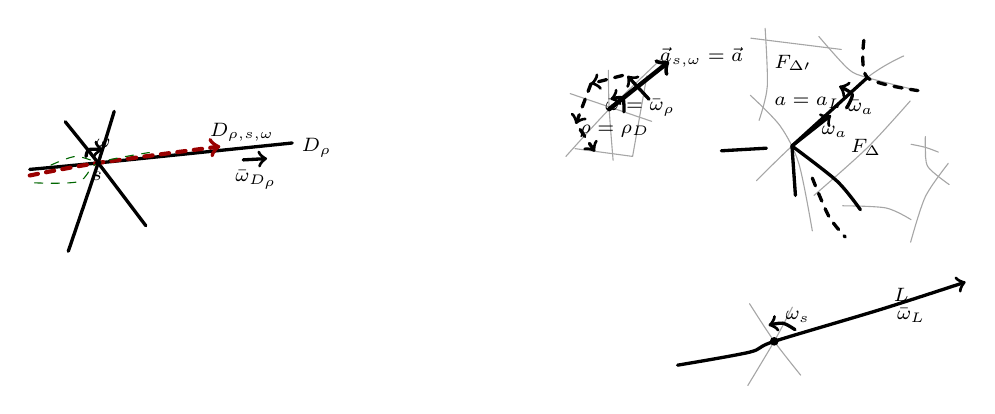
\begin{tikzpicture}[x=.55cm,y=-.55cm,line cap=round,line join=round,g/.style={olive!80!yellow,line width=1.7pt},r/.style={orange!80!brown,line width=1.8pt},w/.style={red!60!black,line width=1.5pt},b/.style={blue!60!black,line width=1.4pt},p/.style={gray!70,thin},k/.style={black,line width=1.2pt},every node/.style={font=\scriptsize}]
% Left local oriented crossing.
\draw[k] plot[smooth] coordinates {(1.43,6.94) (3.01,6.79) (7.49,6.33)};
\draw[k] plot[smooth] coordinates {(2.25,5.84) (3.01,6.79) (4.11,8.24)};
\draw[k] plot[smooth] coordinates {(3.38,5.6) (3.01,6.79) (2.32,8.83)};
\draw[w,dashed,->] plot[smooth] coordinates {(1.43,7.08) (3.01,6.79) (5.83,6.41)};
\draw[green!40!black,dashed] plot[smooth] coordinates {(1.54,7.25) (2.56,7.22) (3.01,6.79) (4.19,6.55)};
\draw[green!40!black,dashed] plot[smooth] coordinates {(1.92,6.84) (2.49,6.64) (3.01,6.79)};
\draw[k,->] plot[smooth] coordinates {(2.73,6.64) (2.8,6.48) (3.12,6.49)};
\draw[k,->] plot[smooth] coordinates {(6.36,6.72) (6.91,6.69)};
\fill[k] (3.01,6.79) circle (.07);
\node at (3.13,6.33) {$\omega$};
\node at (2.98,7.1) {$s$};
\node at (6.33,6.08) {$D_{\unsure{\rho},s,\omega}$};
\node at (8.05,6.44) {$D_\rho$};
\node at (6.66,7.18) {$\bar\omega_{D_\rho}$};
% Central local arrow with orientation and faint construction.
\draw[p] plot[smooth] coordinates {(13.81,6.64) (14.81,5.55) (16.02,4.38)};
\draw[p] plot[smooth] coordinates {(13.91,5.19) (15.79,5.83)};
\draw[p] plot[smooth] coordinates {(14.79,4.65) (14.81,5.55) (14.9,6.73)};
\draw[p] plot[smooth] coordinates {(15.68,4.78) (15.35,6.64)};
\draw[p] plot[smooth] coordinates {(14.02,6.46) (15.35,6.64)};
\draw[k,->,line width=1.6pt] plot[smooth] coordinates {(14.81,5.55) (16.19,4.45)};
\draw[k,->] plot[smooth] coordinates {(15.73,5.32) (15.23,4.78)};
\draw[k,->] plot[smooth] coordinates {(15.15,5.61) (15.12,5.29) (14.84,5.32)};
\draw[k,dashed,->] plot[smooth] coordinates {(15.12,4.77) (14.39,4.96)};
\draw[k,dashed,->] plot[smooth] coordinates {(14.39,4.96) (14.04,5.89)};
\draw[k,dashed,->] plot[smooth] coordinates {(14.14,6.02) (14.48,6.53)};
\node at (16.94,4.35) {$\vec a_{s,\omega}=\vec a$};
\node at (15.52,5.52) {$\bar\omega=\bar\omega_\rho$};
\node at (14.93,6.05) {$\rho=\unsure{\rho_D}$};
% Oriented edge a_L between two face regions.
\draw[p] plot[smooth] coordinates {(18.08,3.91) (20.17,4.17)};
\draw[p] plot[smooth] coordinates {(18.41,3.68) (18.46,5.02) (18.27,5.81)};
\draw[p] plot[smooth] coordinates {(18.07,5.23) (18.76,5.94) (19.19,6.81) (19.5,8.36)};
\draw[p] plot[smooth] coordinates {(19.65,3.87) (20.33,4.62) (20.77,4.82) (21.94,5.12)};
\draw[p] plot[smooth] coordinates {(18.21,7.2) (19.03,6.4) (20.77,4.82) (21.61,4.32)};
\draw[p] plot[smooth] coordinates {(19.54,7.54) (20.77,6.44) (21.76,5.36)};
\draw[p] plot[smooth] coordinates {(20.2,7.78) (21.2,7.83) (21.78,8.1)};
\draw[p] plot[smooth] coordinates {(21.77,8.62) (22.11,7.57) (22.64,6.8)};
\draw[p] plot[smooth] coordinates {(21.78,6.36) (22.11,6.43) (22.41,6.54)};
\draw[p] plot[smooth] coordinates {(22.11,6.18) (22.11,6.43) (22.17,6.88) (22.66,7.29)};
\draw[k] plot[smooth] coordinates {(19.03,6.4) (20.77,4.82)};
\draw[k] plot[smooth] coordinates {(19.03,6.4) (19.11,7.54)};
\draw[k] plot[smooth] coordinates {(19.03,6.4) (20.07,7.21) (20.61,7.87)};
\draw[k] plot[smooth] coordinates {(17.4,6.51) (18.44,6.45)};
\draw[k,dashed] plot[smooth] coordinates {(20.69,3.96) (20.77,4.82) (21.94,5.12)};
\draw[k,dashed] plot[smooth] coordinates {(19.5,7.14) (19.88,8.02) (20.26,8.5)};
\draw[k,->] plot[smooth] coordinates {(19.03,6.4) (19.93,5.69)};
\draw[k,->] plot[smooth] coordinates {(20.29,5.52) (20.42,5.21) (20.12,5.02)};
\node at (19.05,4.48) {$F_{\Delta\prime}$};
\node at (20.74,6.43) {$F_{\Delta}$};
\node at (19.41,5.4) {$a=a_L$};
\node at (20.62,5.51) {$\bar\omega_a$};
\node at (20.01,6.07) {$\omega_a$};
% Oriented L with point s and local rotation omega_s.
\draw[p] plot[smooth] coordinates {(18.05,10.04) (18.62,10.91) (19.23,11.69)};
\draw[p] plot[smooth] coordinates {(19.04,10.12) (18.62,10.91) (18.01,11.93)};
\draw[k,->] plot[smooth] coordinates {(16.39,11.46) (18.05,11.16) (18.62,10.91) (21.09,10.17) (23.04,9.54)};
\draw[k,->] plot[smooth] coordinates {(19.1,10.64) (18.82,10.49) (18.49,10.54)};
\fill[k] (18.62,10.91) circle (.1);
\node at (19.16,10.34) {$\omega_s$};
\node at (21.55,9.84) {$L$};
\node at (21.78,10.32) {$\bar\omega_L$};
\end{tikzpicture}}

La difficulté conceptuelle n'est pas dans l'étude locale de $X^*$ en \unsure{un vois.} de $\rho$, en termes de $D$, mais dans l'étude locale de $X^*$ au voisinage d'une face, correspondant à une p.r. stble $\Delta$, mais dans la description de $X^*$ au voisinage d'une \uline{arête} \inserted{$a_L$}, correspondant à une position r. semi-stble donnée, soit $L$.
Il n'y a pas non plus de difficulté : \unsure{saisir} les faces incidentes \deleted{\unsure{la face} $F$} à $a_L$, et leur circuit des arêtes (contenant $a_L$), mais par contre : saisir les deux \inserted{(?)} sommets incidents à $a_L$.

Notons que la donnée d'une orientation \unsure{superficielle} le long de $a_L$ revient à celle d'une orientation de $L$, celle d'une orientation de $a_L$ à celle d'une orientation superficielle en le \deleted{point} sommet $s\in S_L$, donc une \uline{rive} de $L$\deleted{$\unsure{\{s\}}$} en $s$ revient à celle d'une rive de $a$ i.e. d'une des faces incidentes \unsure{à a}.

Il s'agirait donc, en termes de $(L,\omega_s)$, de reconstruire le sommet extrémité de $\vec a=(a,\omega_a)$, \deleted{\unsure{dans des termes}} si possible en termes d'une position relative critique, déduite de $L$ par ``blocage'' autour de $s$, dans le sens indiqué par l'orientation $\omega_s$ en $\uline{s}$, i.e. par la rive correspondante de $L-\{s\}$.
L'ennui, c'est qu'il y a plusieurs choix naturels qui viennent à l'esprit, et qu'il n'est pas sûr qu'aucun de ces choix ne marche!

{\ttfamily\unsure{//** CRAY6 0013 - O}}
\unsure{{\scriptsize\begin{tabular}{l}
\texttt{\ CCCCCCCCCC\ \ \ RRRRRRRRRRR\ \ \ AAAAAAAAAA\ \ \ YY\ \ \ \ \ \ \ \ YY\ \ \ 6666666666}\\
\texttt{CCCCCCCCCCCC\ \ RRRRRRRRRRRR\ AAAAAAAAAAAA\ \ YY\ \ \ \ \ \ \ \ YY\ \ 666666666666}\\
\texttt{CC\ \ \ \ \ \ \ \ CC\ \ RR\ \ \ \ \ \ \ \ RR\ AA\ \ \ \ \ \ \ \ AA\ \ YY\ \ \ \ \ \ YY\ \ \ 66\ \ \ \ \ \ \ \ 66}\\
\texttt{CC\ \ \ \ \ \ \ \ \ \ \ \ RR\ \ \ \ \ \ \ \ RR\ AA\ \ \ \ \ \ \ \ AA\ \ \ YY\ \ \ \ YY\ \ \ \ 66}\\
\texttt{CC\ \ \ \ \ \ \ \ \ \ \ \ RR\ \ \ \ \ \ \ \ RR\ AA\ \ \ \ \ \ \ \ AA\ \ \ \ YY\ \ YY\ \ \ \ \ 66}\\
\texttt{CC\ \ \ \ \ \ \ \ \ \ \ \ RRRRRRRRRRRR\ AAAAAAAAAAAA\ \ \ \ \ YYYY\ \ \ \ \ \ 66666666666}\\
\texttt{CC\ \ \ \ \ \ \ \ \ \ \ \ RRRRRRRRRRR\ \ AAAAAAAAAAAA\ \ \ \ \ \ YY\ \ \ \ \ \ \ 666666666666}\\
\texttt{CC\ \ \ \ \ \ \ \ \ \ \ \ RR\ \ \ \ RR\ \ \ \ \ AA\ \ \ \ \ \ \ \ AA\ \ \ \ \ \ YY\ \ \ \ \ \ \ 66\ \ \ \ \ \ \ \ 66}\\
\texttt{CC\ \ \ \ \ \ \ \ \ \ \ \ RR\ \ \ \ \ RR\ \ \ \ AA\ \ \ \ \ \ \ \ AA\ \ \ \ \ \ YY\ \ \ \ \ \ \ 66\ \ \ \ \ \ \ \ 66}\\
\texttt{CC\ \ \ \ \ \ \ \ CC\ \ RR\ \ \ \ \ \ RR\ \ \ AA\ \ \ \ \ \ \ \ AA\ \ \ \ \ \ YY\ \ \ \ \ \ \ 66\ \ \ \ \ \ \ \ 66}\\
\texttt{CCCCCCCCCCCC\ \ RR\ \ \ \ \ \ \ RR\ \ AA\ \ \ \ \ \ \ \ AA\ \ \ \ \ \ YY\ \ \ \ \ \ \ 666666666666}\\
\texttt{\ CCCCCCCCCC\ \ \ RR\ \ \ \ \ \ \ \ RR\ AA\ \ \ \ \ \ \ \ AA\ \ \ \ \ \ YY\ \ \ \ \ \ \ \ 6666666666}\\
\end{tabular}}}
{\ttfamily ****A\quad END\quad JOB\quad13\quad CRAY6\quad- CRAY OUTPUT -\quad ROOM\quad3.24.18 PM 19 AUG 82\quad R6.PR1\quad SYS JES2\quad JOB\quad13\quad END\quad A****}\\
{\ttfamily ****A\quad END\quad JOB\quad13\quad CRAY6\quad- CRAY OUTPUT -\quad ROOM\quad3.24.18 PM 19 AUG 82\quad R6.PR1\quad SYS JES2\quad JOB\quad13\quad END\quad A****}\\
{\ttfamily ****A\quad END\quad JOB\quad13\quad CRAY6\quad- CRAY OUTPUT -\quad ROOM\quad3.24.18 PM 19 AUG 82\quad R6.PR1\quad SYS JES2\quad JOB\quad13\quad END\quad A****}\\
{\ttfamily ****A\quad END\quad JOB\quad13\quad CRAY6\quad- CRAY OUTPUT -\quad ROOM\quad3.24.18 PM 19 AUG 82\quad R6.PR1\quad SYS JES2\quad JOB\quad13\quad END\quad A****}\\
{\ttfamily ****A\quad END\quad JOB\quad13\quad CRAY6\quad- CRAY OUTPUT -\quad ROOM\quad3.24.18 PM 19 AUG 82\quad R6.PR1\quad SYS JES2\quad JOB\quad13\quad END\quad A****}\\
{\ttfamily ****A\quad END\quad JOB\quad13\quad CRAY6\quad- CRAY OUTPUT -\quad ROOM\quad3.24.18 PM 19 AUG 82\quad R6.PR1\quad SYS JES2\quad JOB\quad13\quad END\quad A****}\\
\margin{\mspage{150}}
